% Source: http://www.brian-amberg.de/uni/poster/
\documentclass[landscape,paperwidth=96in,paperheight=48in,fontscale=0.2]{baposter}
\usepackage[utf8]{inputenc}
\usepackage{fontspec,amsfonts,microtype}
\usepackage{hyperref,url}   % hyperlinks
\usepackage{booktabs}       % professional-quality tables
\usepackage{}      % microtypography
\usepackage{nicefrac,mathtools,xfrac,bm,amsthm}
\usepackage{graphicx}
\usepackage{pgfplots}
\usetikzlibrary{pgfplots.groupplots}
\pgfplotsset{compat=1.18}
\usepackage{tabularx}
\usepackage{comment}
\usepackage{fnpct}
\usepackage{caption}
\usepackage{comment}
\usepackage[framemethod=tikz]{mdframed}

\DeclareMathOperator*{\minimize}{minimize}
\renewcommand{\familydefault}{\sfdefault}

\usepackage{enumitem}\setlist{nolistsep,leftmargin=*}
\usepackage{graphicx}

\usepackage{tikz}
\usetikzlibrary[topaths]
\newcount\mycount

\setmainfont{Lato}[
  SizeFeatures={Size=18},
]
\newfontfamily\titlefont{Raleway-SemiBold}[
  Path = ./fonts/raleway/,
  SizeFeatures={Size=32},
]
\newfontfamily\headerfont{Raleway-Bold}[
  Path = ./fonts/raleway/,
  SizeFeatures={Size=17},
]

\definecolor{headerColor}{rgb}{0.14, .62, .92}


% Display graphics in pgfplots without deformation: https://tex.stackexchange.com/a/338627
\makeatletter
\newcommand\addplotgraphicsnatural[2][]{%
    \begingroup
    % set options in this local group (will be lost afterwards):
    \pgfqkeys{/pgfplots/plot graphics}{#1}%
    % measure the natural size of the graphics:
    \setbox0=\hbox{\includegraphics{#2}}%
    %
    % compute the required unit vector ratio:
    \pgfmathsetmacro{\xfactor}{\wd0/(\pgfkeysvalueof{/pgfplots/plot graphics/xmax} - \pgfkeysvalueof{/pgfplots/plot graphics/xmin})}%
    \pgfmathsetmacro{\yfactor}{\ht0/(\pgfkeysvalueof{/pgfplots/plot graphics/ymax} - \pgfkeysvalueof{/pgfplots/plot graphics/ymin})}\yfactor%
    % The smaller of the unit vectors should be 1, so the other needs to be scaled appropriately
    \pgfmathsetmacro{\xunit}{\xfactor<\yfactor ? 1 : \xfactor/\yfactor}
    \pgfmathsetmacro{\yunit}{\xfactor<\yfactor ? \yfactor/\xfactor : 1}
    %
    % configure pgfplots to use it.
    % The \xdef expands all macros except those prefixed by '\noexpand'
    % and assigns the result to a global macro named '\marshal'.
    \xdef\marshal{%
        \noexpand\pgfplotsset{unit vector ratio*={\xunit\space \yunit}}%
    }%
    \endgroup
    %
    % use our macro here:
    \marshal
    %
    \addplot graphics[#1] {#2};
}   
\makeatother


\begin{document}

\begin{poster}{
    grid=true,
    colspacing=.5in,
    headerColorOne=headerColor, borderColor=headerColor,
    headerborder=none, headershape=rectangle,
    headershade=plain, headerFontColor=white, textborder=none,
    background=plain, bgColorOne=white, boxshade=none,
    headerheight=0.15\textheight,
    headerfont=\headerfont,
    columns=3
  }{
    
\includegraphics[height=0.11\textheight]{images/neurips-logo}
  }{
    {{\titlefont The Pitfalls of Regularization in Off-Policy TD Learning }}
  }{\vspace{2mm}\large
    Gaurav Manek, J. Zico Kolter \\
    School of Computer Science, Carnegie Mellon University \\
    \texttt{<gmanek, zkolter>@cs.cmu.edu}
  }{
\includegraphics[height=0.11\textheight]{images/cmu-logo}}

  \headerbox{Off-Policy TD Learning is Unstable}
  {name=intro,column=0,row=0}{% Highlight Box
\definecolor{teal}{rgb}{0.99,0.37,0.53}
\newmdenv[innerlinewidth=0.5pt, roundcorner=4pt,linecolor=teal,backgroundcolor=teal,innerleftmargin=6pt,
    innerrightmargin=6pt,innertopmargin=6pt,innerbottommargin=6pt,leftmargin=-9pt,rightmargin=-9pt]{mybox}

Temporal Difference (TD) learning estimates the value function of a Markov Reward Process (MRP) using samples of successive differences. This is done with the Bellman equation:
\begin{center}
    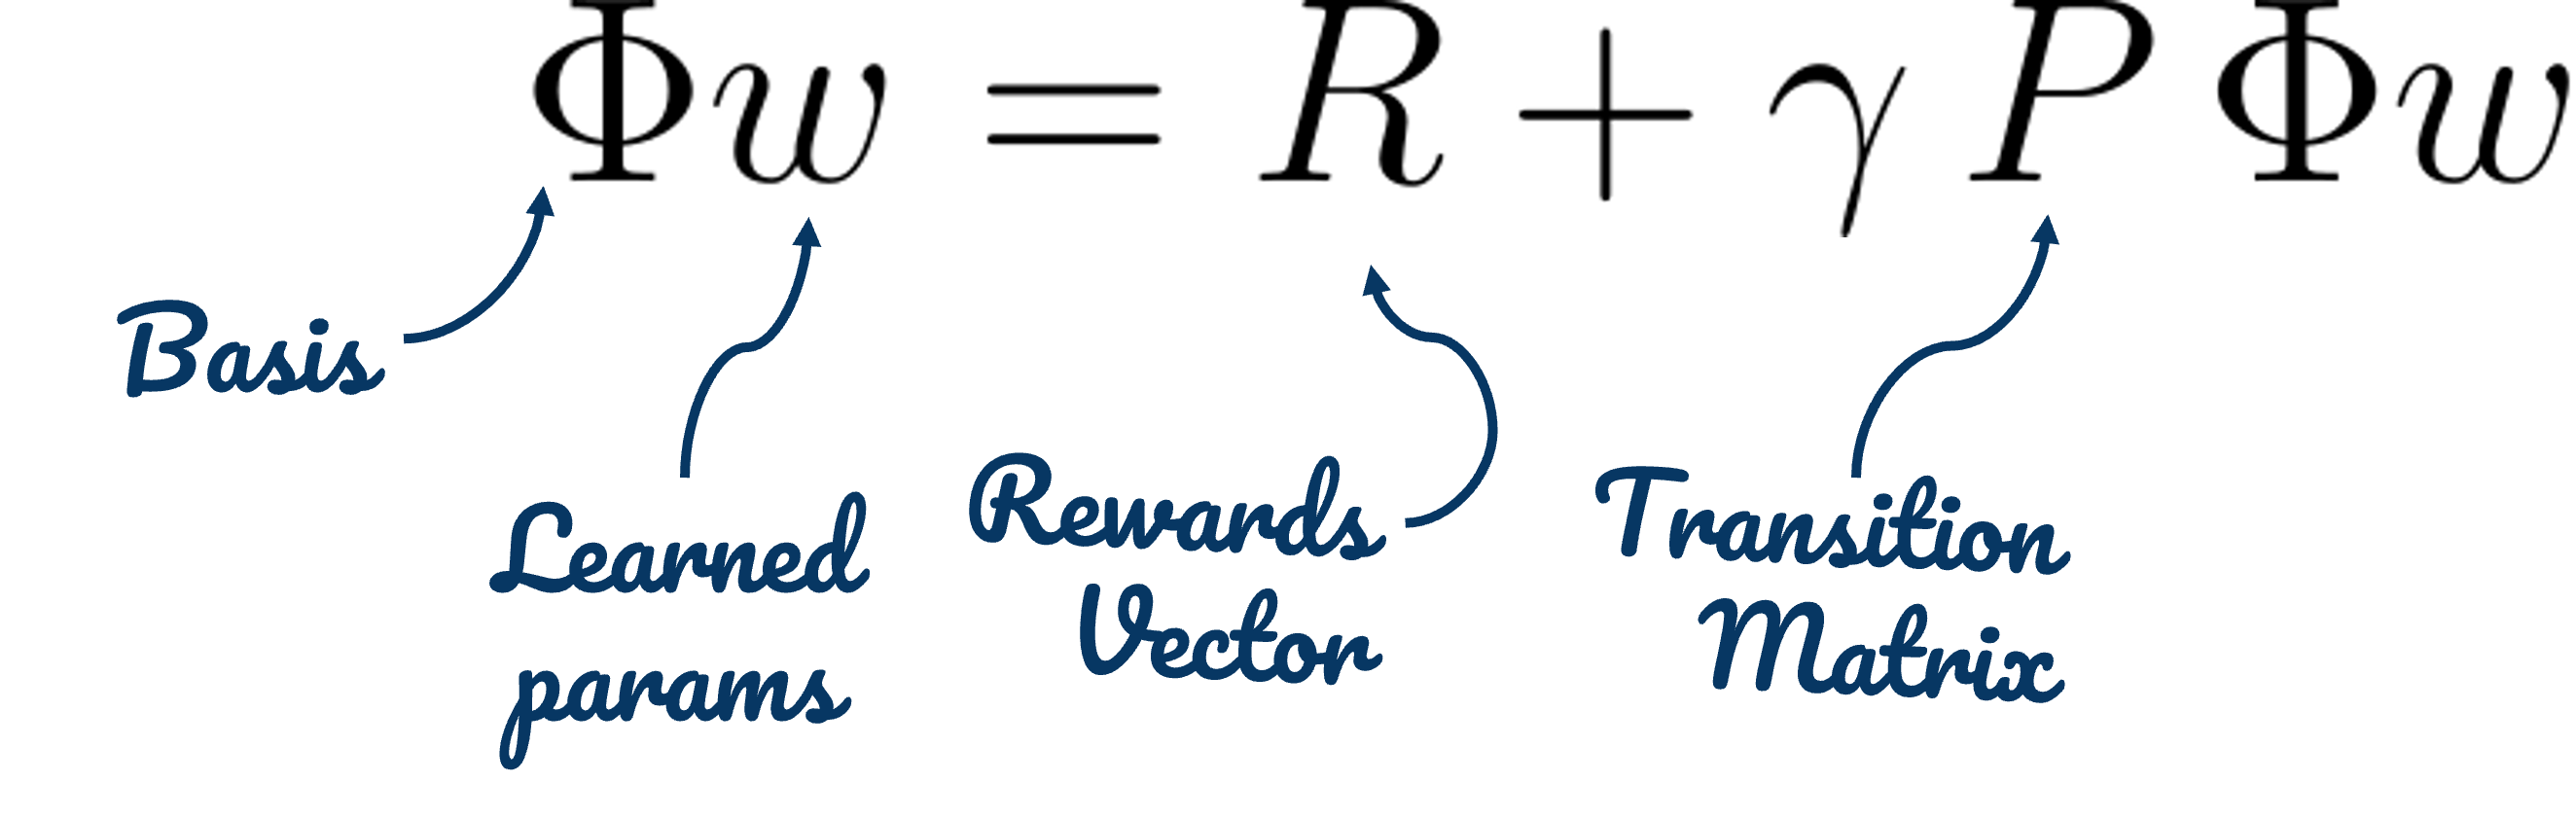
\includegraphics[scale=0.4]{parts/intro/bellman}
\end{center}\vspace{-.1in}
TD may learn arbitrarily bad value functions under \emph{Deadly Triad} conditions:
bootstrapping (learning from your own output),
function approximation, and
off-policy updates.
\vspace{-.11in}
\begin{center}
    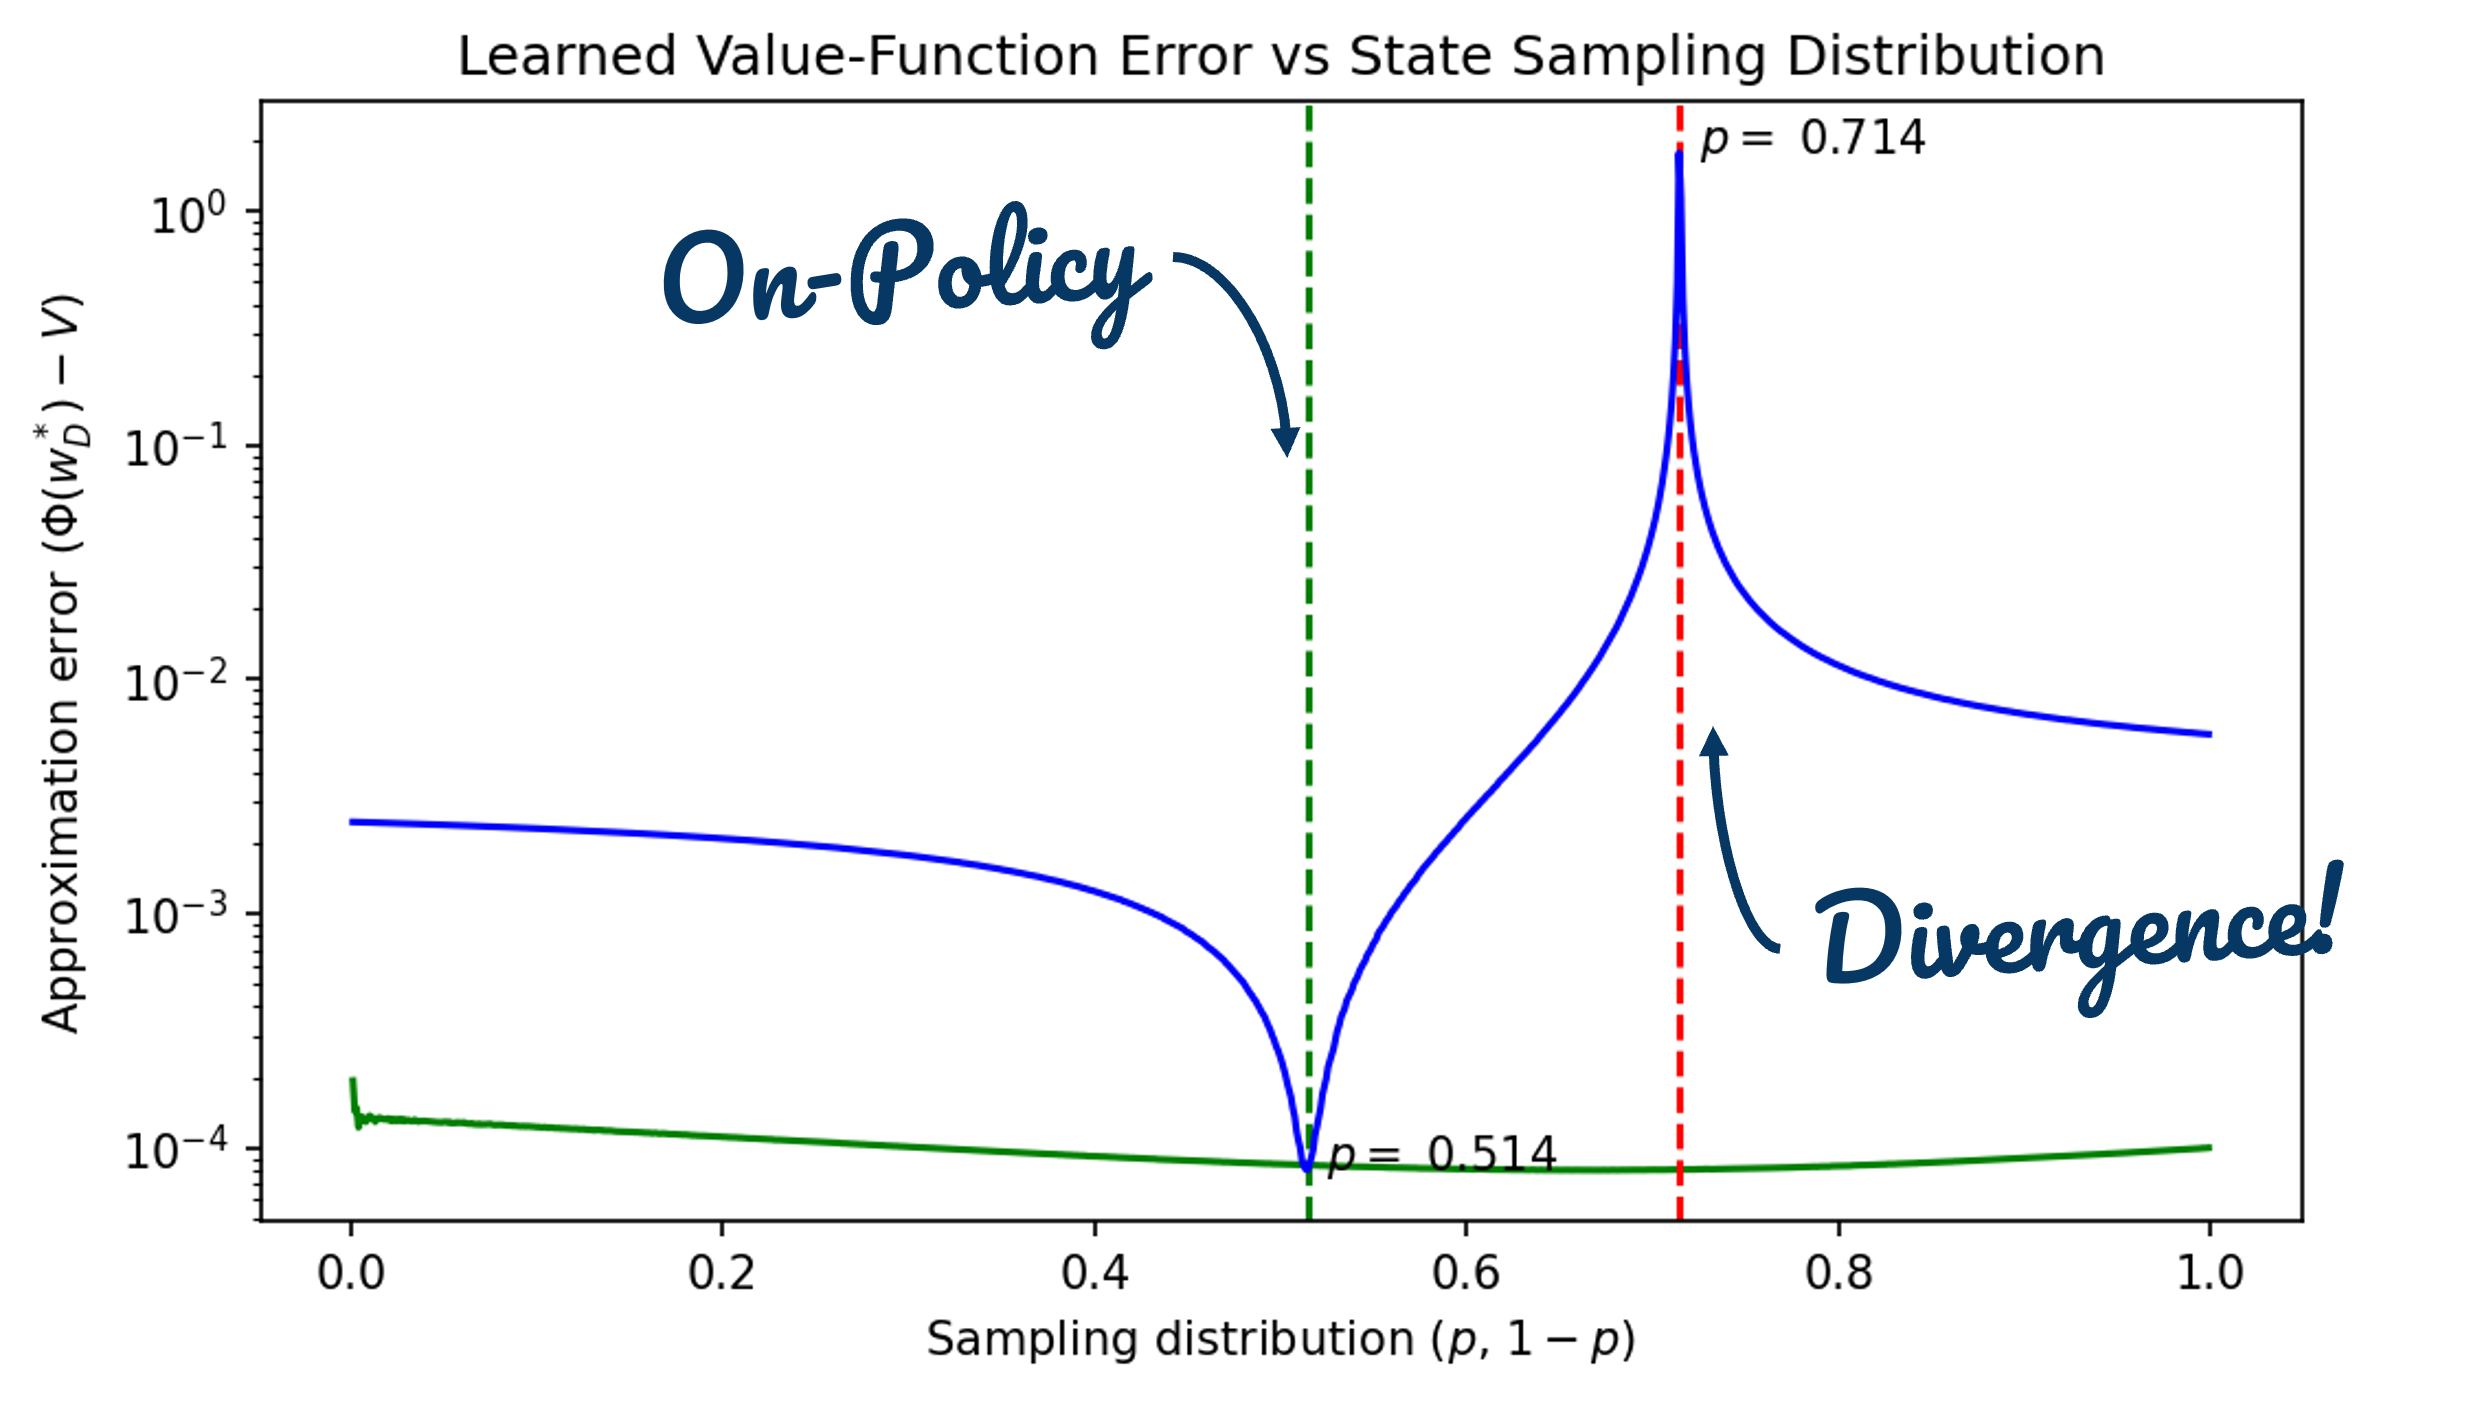
\includegraphics[scale=0.4]{parts/intro/threestatedivergence}
\end{center}\vspace{-.1in}
Regularization is a popular mitigation, and is supposed to work like this:
\begin{center}
    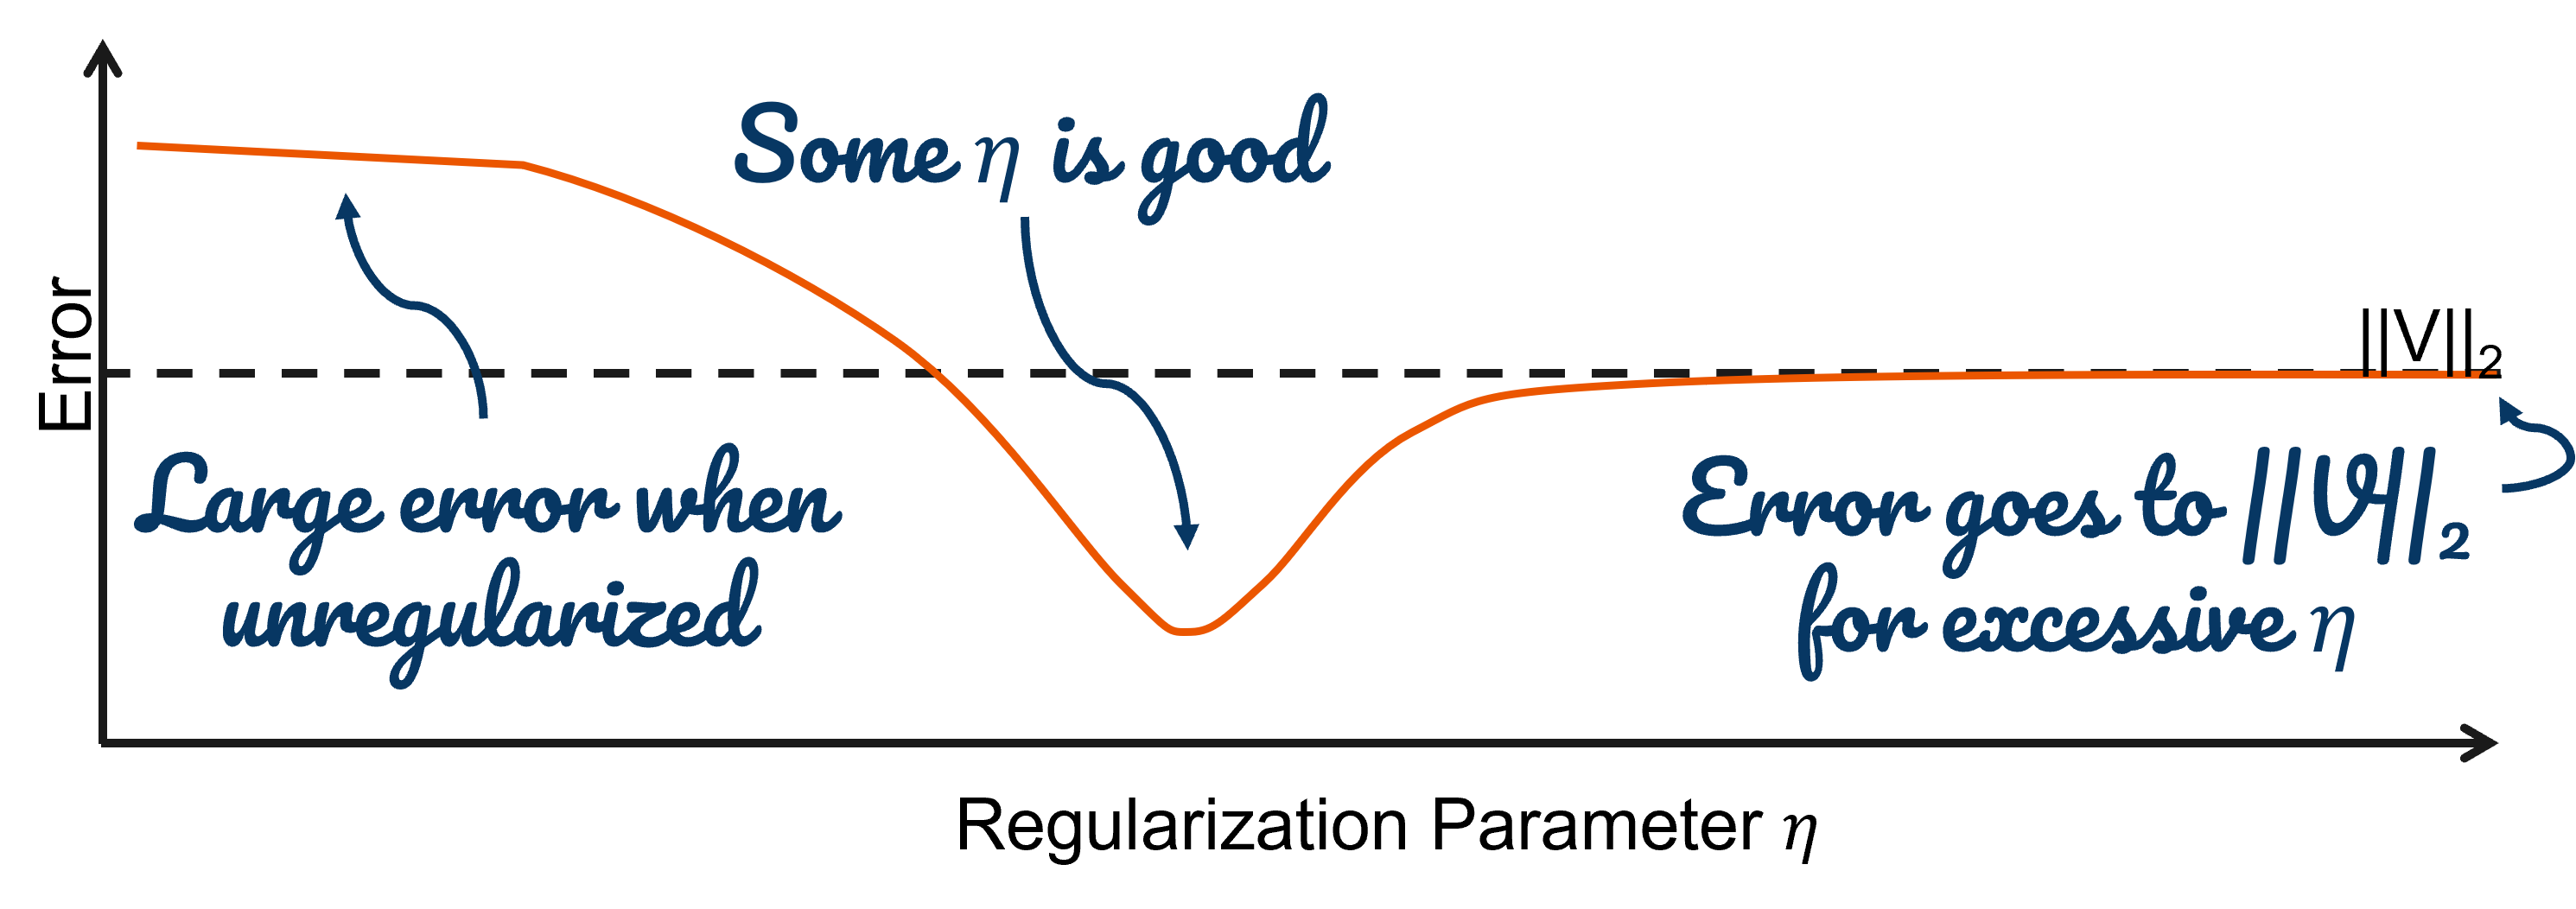
\includegraphics[scale=0.4]{parts/intro/regworks}
\end{center}
\begin{mybox}
    {\headerfont Regularization doesn't always work!}
    \vspace{.5em}
    {\large
        \begin{enumerate}
            \item Models may be \emph{vacuous}.
            \item Regularizing TD is \emph{not monotonic}.
            \item Emphatic models are \emph{not immune}.
        \end{enumerate}
    }
    \vspace{.5em}
\end{mybox}}

  \headerbox{Example \#1: Models may be \textit{vacuous}}
  {name=randomnet,column=1,row=0}{% Highlight Box
oral Difference (TD) learning is the process of estimating the value of each state using the differences in the value of successive states. This is done with the Bellman equation:
\begin{center}
    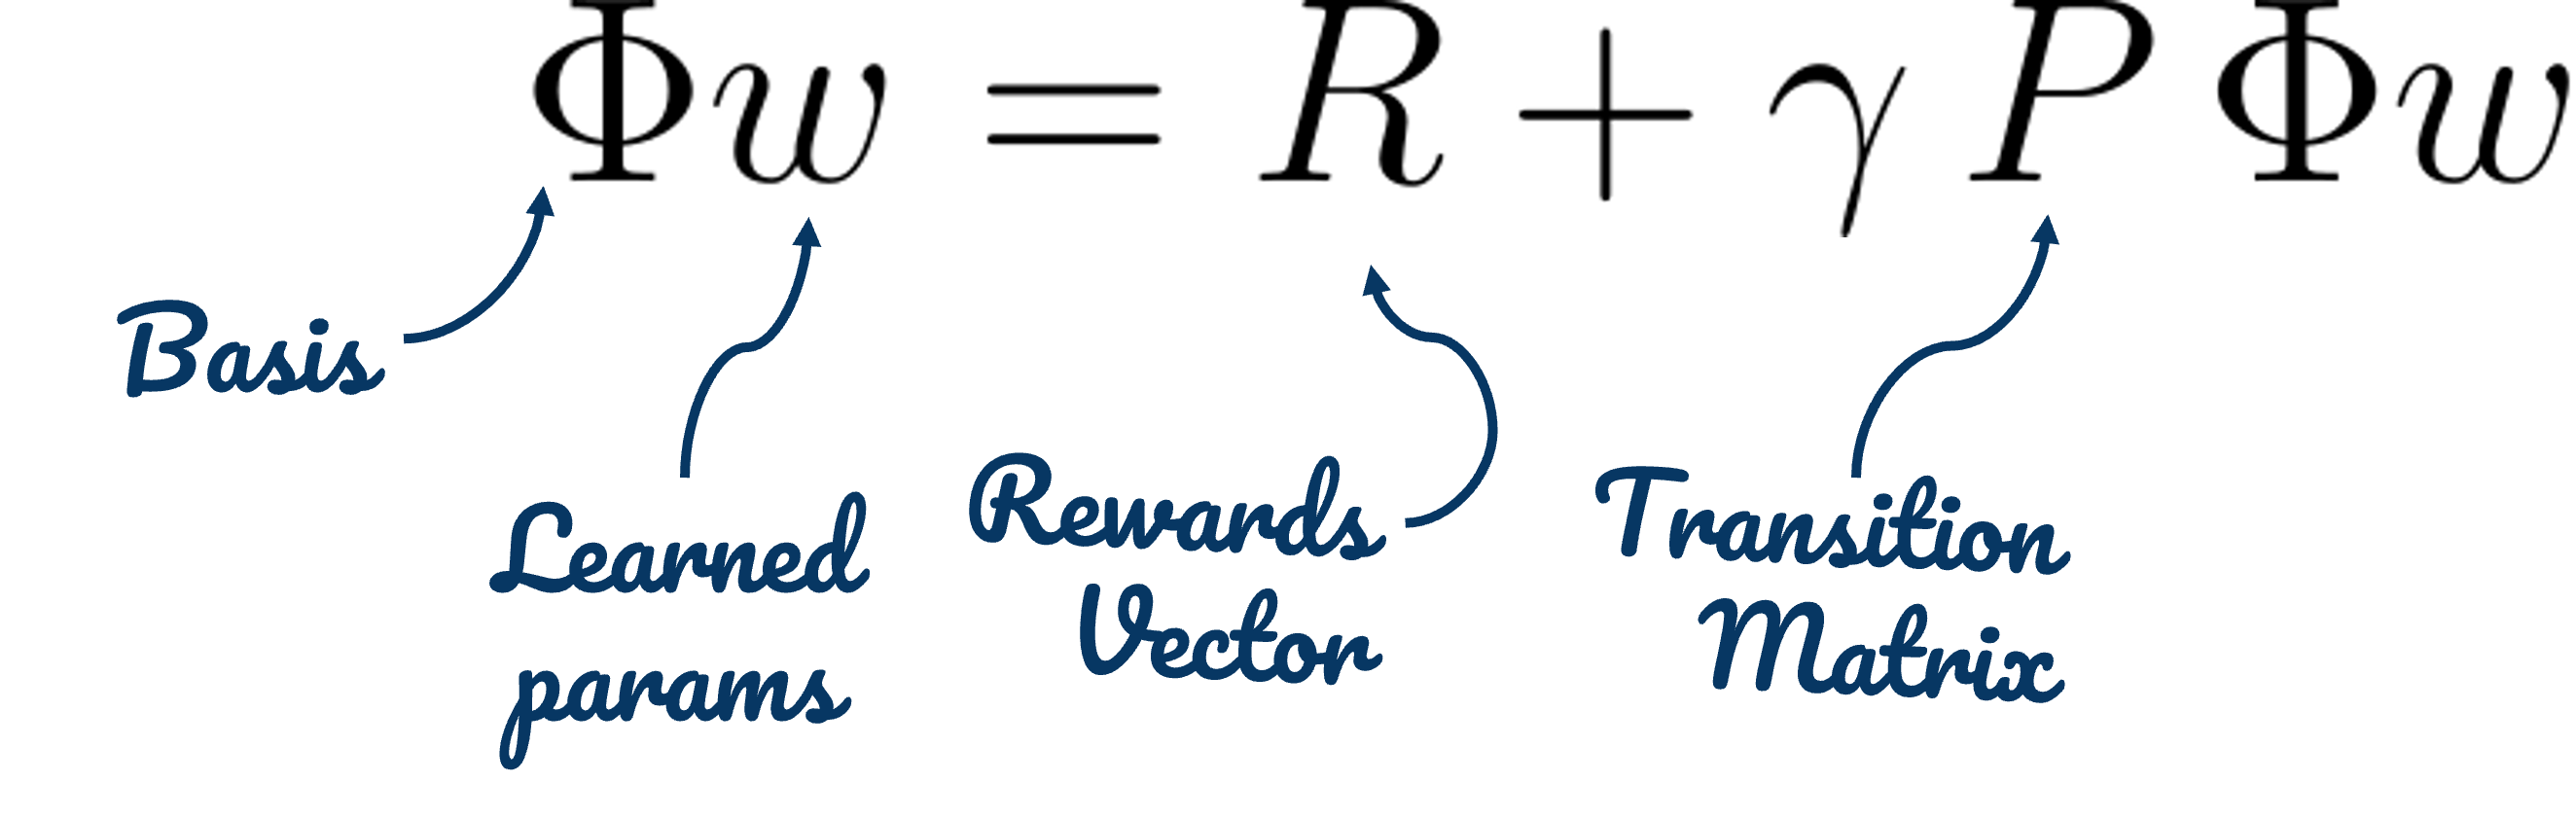
\includegraphics[scale=0.4]{parts/intro/bellman}
\end{center}
TD may learn arbitrarily bad value functions under the \emph{Deadly Triad} conditions:
}

  %\headerbox{Empirical Result: Damped Pendulum}
  %{name=pendulum,column=2,row=0}{\input{pendulum}}

  %\headerbox{Empirical Result: Damped $n$-link Pendulum}
  %{name=nlinkpendulum,column=2,below=pendulum}{\input{nlinkpendulum}}


\end{poster}
\end{document}
